\chapter{\IfLanguageName{dutch}{Stand van zaken}{State of the art}}
\label{ch:stand-van-zaken}

% Tip: Begin elk hoofdstuk met een paragraaf inleiding die beschrijft hoe
% dit hoofdstuk past binnen het geheel van de bachelorproef. Geef in het
% bijzonder aan wat de link is met het vorige en volgende hoofdstuk.

% Pas na deze inleidende paragraaf komt de eerste sectiehoofding.
\section{\IfLanguageName{dutch}{Global Positioning System (GPS)}{Global Positioning System (GPS)}}
Het Global Positioning System is een wereldwijd gekend systeem, maar toch zijn er heel wat verschillen. Als er gesproken wordt over GPS, wordt er impliciet NAVSTAR bedoeld.\autocite{gps} Dit eerste operationele GPS-systeem had oorspronkelijk enkel militaire toepassingen. Het is ontwikkeld door de 'United States Air Force'. \autocite{gnss}  Later is NAVSTAR toegankelijk gemaakt voor de gewone gebruiker. In deze sectie wordt toegelicht welke de verschillende systemen zijn en welke gebruikt kunnen worden.

\subsection{\IfLanguageName{dutch}{De werking van GPS}{How GPS works}}
\begin{figure}
	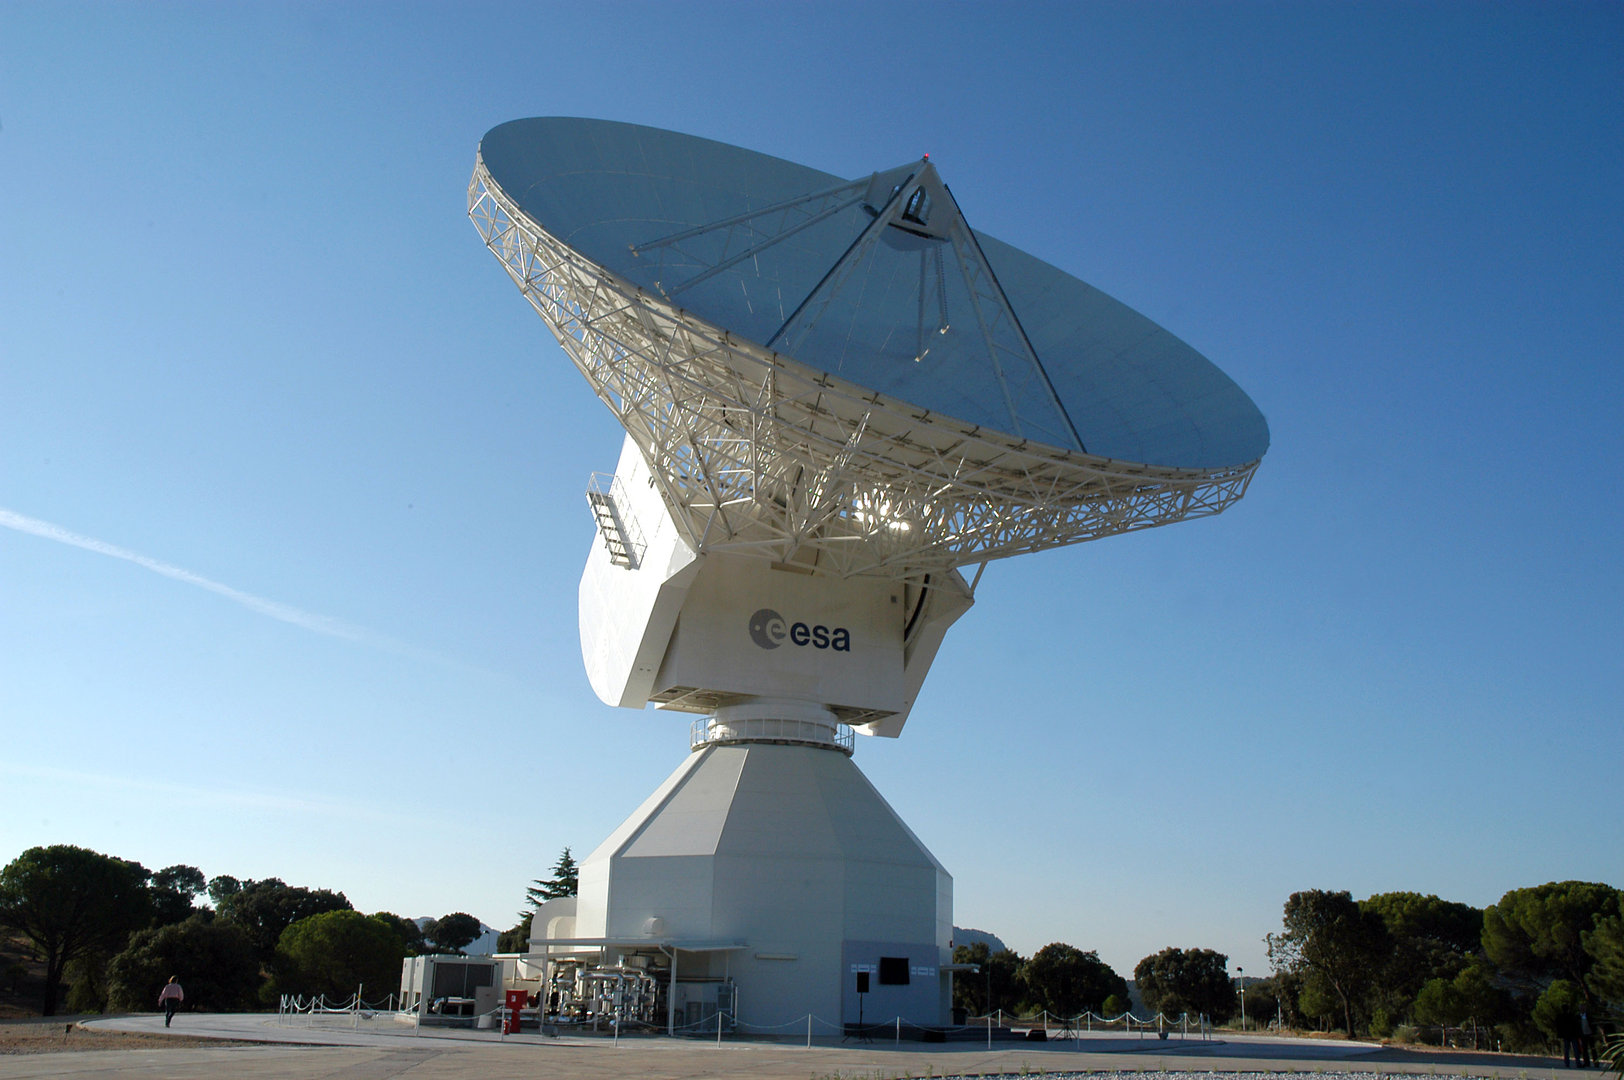
\includegraphics[width=\textwidth,height=\textheight,keepaspectratio]{groundstation.jpg}
	%https://www.google.com/url?sa=i&url=https%3A%2F%2Fwww.esa.int%2FAbout_Us%2FESAC%2FCebreros_ground_station&psig=AOvVaw3m4fRPzsoJEUD7uxKB9P8U&ust=1583062350499000&source=images&cd=vfe&ved=0CAMQjB1qFwoTCJD8uPrU9ucCFQAAAAAdAAAAABAD
	\caption[Voorbeeld grondstation]{\href{https://www.esa.int/About_Us/ESAC/Cebreros_ground_stationt}{Voorbeeld grondstation}}
	\label{fig:groundstation}
\end{figure}
\begin{figure}
	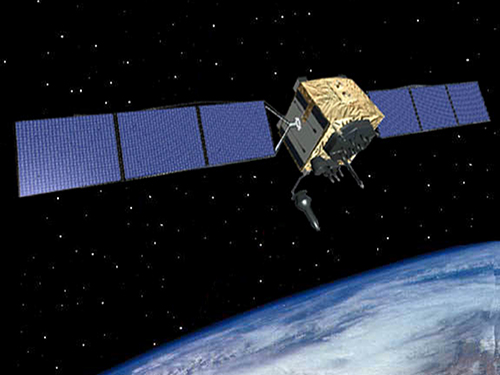
\includegraphics[width=\textwidth,height=\textheight,keepaspectratio]{satelliet.jpg}
	%https://www.google.com/url?sa=i&url=https%3A%2F%2Fspacenews.com%2F40530gps-2f-6-navigation-satellite-slated-to-launch-on-may-15%2F&psig=AOvVaw0tzOggmMim-1CxoYTRl1Ze&ust=1583062792344000&source=images&cd=vfe&ved=0CAMQjB1qFwoTCOD3jc3W9ucCFQAAAAAdAAAAABAD
	\caption[Voorbeeld GPS-satelliet]{\href{https://spacenews.com/40530gps-2f-6-navigation-satellite-slated-to-launch-on-may-15/}{Voorbeeld GPS-satelliet}}
	\label{fig:satelliet}
\end{figure}

Het doel van een GPS is om te navigeren. Daarvoor moet de locatie heel nauwkeurig bepaald worden. Hiervoor zijn drie zaken nodig:
\begin{itemize}
	\item Grondstation, deze zijn ontworpen voor buitenplanetaire\footnote[1]{De ruimte buiten onze planeet} draadloze communicatie. Ze communiceren door het ontvangen en verzenden van radiogolven met zeer hoge frequentie. (Zie figuur: \ref{fig:groundstation})
	\item Een satelliet, of ook vaak kunstmaan genoemd, is een object dat zich in een baan om een hemellichaam bevindt. \autocite{definitie_satelliet} (Zie figuur: \ref{fig:satelliet})
	\item GPS-ontvanger, dit ontvangt de elektromagnetische signalen van de satellieten.
\end{itemize}

De grondstations worden gebruikt om de locatie bij te houden van de GPS-satellieten. Deze stations worden niet gebruikt voor het bepalen van de huidige locatie van een gebruiker. 
\newline
\newline
De GPS-satellieten zenden een signaal uit die de afstand en tijd bevat. Deze tijd wordt berekend met een klok aan boord. Een kwartskristalklok kan na 6 weken een volledige milliseconde afwijken van de werkelijke tijd door temperatuurschommelingen. Dit is gevaarlijk omdat het een grote impact heeft op het opmeten van posities bij snel bewegend ruimtevaartuig. Hierdoor maken satellieten gebruik van een ander type klok, de atoomklok. Atoomklokken zijn een 'verbetering' ten opzichte van de kwartskristal klok.  Na 10 jaar wijkt een atoomklok slechts een microseconde af, wat stabieler is in vergelijking met de kwartskristal klok. Alles moet stabiel blijven voor ruimtevaartmisies, waardoor de afwijking van de atoomklok dagelijks gecorrigeerd wordt. \autocite{atomic_clock}
\newline
Als de GPS-ontvanger de tijd en afstand uit het signaal heeft kunnen afleiden, kan het aan de hand van triangulatie zijn locatie bepalen. (Zie figuur: \ref{fig:triangulatie})
Per satelliet wordt een radius bepaald. Hiervoor zijn minstens drie satellieten nodig. De overlapping van de radiussen bepalen één punt, de locatie van de GPS-ontvanger. Soms kan dit niet accuraat gebeuren, waarbij de radius van een vierde satelliet kan helpen. De laatste radius sluit dan foute mogelijkheden uit waardoor de locatie accurater is. Er is met andere woorden een positieve correlatie tussen het aantal satellieten dat gebruikt wordt en de nauwkeurigheid van de locatiebepaling. \autocite{gps}

\begin{figure}
	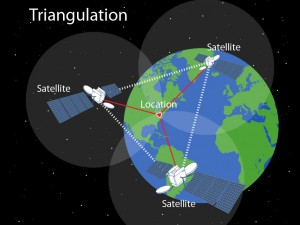
\includegraphics[width=\textwidth,height=\textheight,keepaspectratio]{triangulatie.jpg}
	%https://www.google.com/url?sa=i&url=https%3A%2F%2Fcommunicatiekc.com%2Ftriangulatie%2F&psig=AOvVaw3yrDqiAvEq65KAYiid2aw6&ust=1583063314296000&source=images&cd=vfe&ved=0CAMQjB1qFwoTCKCi68bY9ucCFQAAAAAdAAAAABAD
	\caption[Werking triangulatie]{\href{https://www.youtube.com/watch?v=QK1lDsinMwk}{Visualisatie hoe triangulatie werkt.}}
	\label{fig:triangulatie}
\end{figure} 
\pagebreak
\subsection{\IfLanguageName{dutch}{Global Navigation Satellite Systems (GNSS)}{Global Navigation Satellite Systems (GNSS)}}
Als er gesproken wordt over het bepalen van een locatie, gebruiken we systematisch de term 'GPS'. \autocite{gnss} Dit is echter niet correct, want er bestaan veel meer technologieën en systemen die hierbij helpen. Deze technologieën worden besproken in dit hoofdstuk.
\newline
Het 'Global Positioning System' is een 'ruimte gebaseerd' navigatiesysteem dat eigendom is van de Verenigde Staten en bestuurd wordt door de 'United States Air Force' (USAF). Officieel heet dit systeem 'Navigation Satellite Time And Ranging' (NAVSTAR). De allereerste versie werd gelanceerd in 1978 en in 1995 werd het operationeel verklaard. GPS is in staat om een ongelimiteerd gebruikers met een GPS-ontvanger te voorzien van hun locatie op ieder moment van de dag, onafhankelijk van het weer en over de hele wereld. \autocite{gps}
\newline
Naast NAVSTAR bestaat er ook:
\begin{itemize}
	\item Galileo, beheerd door de Europese Unie (EU).
	\item Globalnaya navigatsionnaya sputnikovaya sistema (GLONASS), beheerd door Rusland.
	\item BeiDou Navigation Satellite System (BDS), beheerd door China, ook Compass genoemd.
	\item Indian Regional Navigation Satellite System (IRNSS/NavIC), beheerd door India.
	\item Quasi-Zenith Satellite System (QZSS), beheerd door Japan
\end{itemize}

Er zijn verschillen tussen tussen deze Global Navigation Satellite Systems, namelijk de accuraatheid en het aantal satellieten. QZSS en IRNSS zijn niet ontworpen als globale GPS-systemen. (Zie tabel:\ref{tab:GNSS-vergelijking})
\begin{table}[]
	\begin{tabular}{lll}
		Systeem & Aantal satellieten (actief) & Nauwkeurigheid                                                                        \\
				BDS     & 35                          & 3.6 meter                                                                      \\
		NAVSTAR & 31                          & 3-5 meter                                                                             \\
		GLONASS & 24+                         & 4-10 meter                                                                            \\
		Galileo & 24+                         & 20-50 centimeter                                                                      \\
		IRNSS   & 7                           & \textless 10 meter over India en \textgreater{}20 meter over de Indische Oceaan regio \\
		QZSS    & 7                           & 1 - 0,01 meter                                                                       
	\end{tabular}
\label{tab:GNSS-vergelijking}
\caption{Overzicht Global National Satellite Systems}
\autocite{gnss}
\end{table}
\newline
De reden voor het bestaan van deze verschillende systemen is van politieke aard. De EU en Rusland wilden niet afhankelijk zijn van de Verenigde Staten (NAVSTAR).

\section{Verschillende Locatiebepaling-technologieën}
\label{sec:Locatiebepaling-technologieën}
Het bepalen van een positie kan op veel manieren gebeuren. De systemen die besproken werden in de vorige sectie vallen allemaal terug op de traditionele methode, triangulatie. De werking van deze methode wordt in deze sectie verder toegelicht. Naast de traditionele methode is het belangrijk om te weten welke andere opties er nog bestaan. Er is onderzoek gedaan naar alle locatiebepaling-technologieën om de meest accurate technologie te bepalen die gebruikt kan worden door de proof of concept. Naast de accuraatheid moet ook de locatiebepaling op zoveel mogelijk plaatsen succesvol werken zodat de proof of concept gebruikt kan worden als lawinepieper in de bergen of als GPS-tracker aan een kust.

\subsection{\IfLanguageName{dutch}{Standard Positioning Service (SPS)}{Standard Positioning Service (SPS)}}
De 'Standard Positioning Service' (SPS) is een positionerings- en timingdienst die signalen broadcast op de GPS L1-frequentie. Deze frequentie, die gebruikt wordt door alle  \mbox{NAVSTAR} GPS-satellieten, zorgt ervoor dat GPS vrij te gebruiken is voor iedereen. \autocite{gps}
\newline
Deze vorm van GPS minder accuraat in vergelijking met het 'Precision Positioning Service'. 
\subsection{\IfLanguageName{dutch}{Precision Positioning Service (PPS)}{Precision Positioning Service (PPS)}}
De 'Precision Positioning Service' (PPS) is een  positionerings- en timingdienst die signalen broadcast op de GPS L1 en L2 frequenties. Het functioneert hetzelfde als SPS, maar hierbij wordt er ook gebruik gemaakt van een precisiecode (P) die alleen beschikbaar is voor geautoriseerde gebruikers. Hiermee wordt voornamelijk het Amerikaans leger en zijn allianties bedoeld. \autocite{pps} Voor september 2007 werd er gebruik gemaakt van 'Selective Availability' (SA). Zo kon het leger van de Verenigde Staten de accuraatheid bewust degraderen voor veiligheidsredenen. De nieuwere GPS III-satellieten zouden niet meer uitgerust zijn met de SA-functie. 
\newline
Deze service wordt voor de proof of concept niet gebruikt omdat het  ontoegankelijk is voor gewone burgers.
\subsection{\IfLanguageName{dutch}{Differential Global Positioning System (DGPS)}{Differential Global Positioning System (DGPS)}}
Differential Global Positioning System (DGPS) verbetert de accuraatheid van GPS. Dit systeem maakt gebruik van correctietechnieken. Deze technieken kunnen real-time gebeuren of ook na het bepalen van de locatie. DGPS vereist een GPS-ontvanger (referentiestation/basisstation) waarvan de locatie gekend is (fixed). De referentie gaat zijn locatie herberekenen en berekent het verschil tussen de gekende locatie en de berekende locatie. Het verschil wordt als volgt toegepast op de GPS-ontvanger zijn berekende locatie. Deze techniek resulteert in een betere locatiebepaling voor de tweede GPS-ontvanger. \autocite{dgps} (Zie figuur:\ref{fig:dgps})
\begin{figure}
	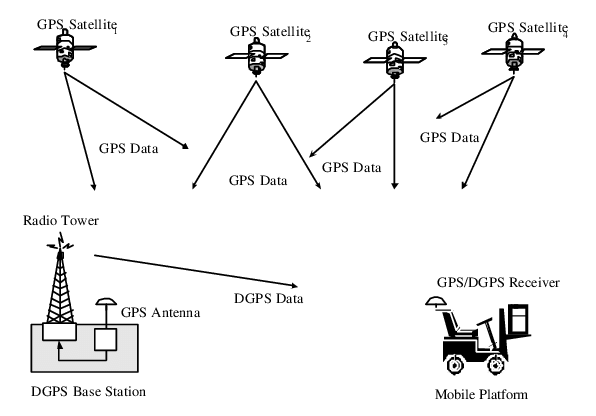
\includegraphics[width=\textwidth,height=\textheight,keepaspectratio]{dgps.png}
		%https://www.google.com/url?sa=i&url=https%3A%2F%2Fwww.researchgate.net%2Ffigure%2FComponents-of-a-DGPS-System_fig1_252064818&psig=AOvVaw07YsVmaU9ifoTgAxmkFPSb&ust=1583073831676000&source=images&cd=vfe&ved=0CAMQjB1qFwoTCPCjlt7_9ucCFQAAAAAdAAAAABAD
	\caption[Differential Global Positioning System]{\href{https://www.researchgate.net/figure/Components-of-a-DGPS-System_fig1_252064818}{Na het bepalen van de locatie via satellieten, ontvangt de GPS-ontvanger correcties van een DGPS station}}
	\label{fig:dgps}
\end{figure}
\newline
De 'Flemish Positioning Service' (FLEPOS) maakt eveneens gebruik van deze techniek. Het FLEPOS 3.0-netwerk bestaat momenteel uit 45 GNSS-referentiestations, waarvan 33 referentiestations in eigen beheer. Het gebruik hiervan is gratis indien de aanvraag voor een abonnement is goedgekeurd. Deze referentiestations bevinden zich in België, Nederland, Frankrijk, Duitsland en Engeland.
\newline
Door het beperkt aantal referentiestations kan deze methode niet geïmplementeerd worden binnen de proof of concept, omdat het bereik niet globaal genoeg is.
\subsection{\IfLanguageName{dutch}{Wide Area Augmentation System (WAAS)}{Wide Area Augmentation System (WAAS)}}
'Wide Area Augmentation' (WAAS) kan, naast basisstation op aarde (DGPS), ook GEO-satellieten gebruiken als vaste referentiepunten. Deze satellieten bevinden zich op 36.000 km hoogte boven de evenaar en draaien rond op dezelfde snelheid als de aarde. Hierdoor blijft de positie van de geosatelliet stationair ten opzichte van de aarde, waardoor het gebruikt kan worden als referentiestation.(Zie figuur:\ref{fig:geostationair})
\begin{figure}
	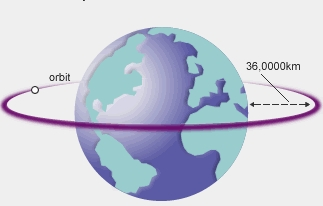
\includegraphics[width=\textwidth,height=\textheight,keepaspectratio]{geostationair.png}
	%https://aardrijkskunde.dbz.be/graad3/taken/oefening_satellieten.htm
	\caption[Geostationair]{\href{https://aardrijkskunde.dbz.be/graad3/taken/oefening_satellieten.htm}{De hoogte waarin satellieten zich moeten bevinden om geostationair te zijn}}
	\label{fig:geostationair} 
\end{figure}
\subsection{\IfLanguageName{dutch}{Assisted Global Positioning System (A-GPS)}{Assisted Global Positioning System (A-GPS)}}
Een GPS-toestel kan er enkele minuten over doen om een locatie te bepalen. Deze verloren tijd heet 'Time To First Fix' (TTFF). De duur van deze TTFF hangt af van de exacte locatie en storing. Een open veld zal een kleinere TTFF hebben dan een bebouwde oppervlakte. Assisted Global Positioning (AGPS/A-GPS/aGPS) verkleint de TTFF. 
\newline
Gsm-masten hebben GPS-ontvangers die voortdurend informatie van GPS-satellieten verzamelen. Op deze informatie worden allerlei bewerkingen uitgevoerd en vervolgens opgeslagen in een database. Dit heeft enkele voordelen voor de gsm die zijn locatie probeert te bepalen:
\begin{itemize}
	\item Snellere locatie bepaling;
	\item Minder computerkracht nodig;
	\item Minder batterijverbruik;
	\item Mogelijkheid om de locatie indoor te bepalen.
\end{itemize} 
Opmerkelijk is dat de accuraatheid minder goed is in vergelijking met het zelf bepalen van de locatie (Zie: \ref{tab:GNSS-vergelijking}). Er zullen field tests en metingen worden uitgevoerd om deze stellingen te controleren. \autocite{agps}
\subsection{\IfLanguageName{dutch}{Advanced Mobile Location (AML)}{Advanced Mobile Location (AML)}}
Tot nu toe was er nog geen enkele techniek die een exacte locatie kon bepalen. 'Advanced Mobile Location' (AML) is de nieuwste (open source) techniek die hiervoor een oplossing biedt. Het maakt gebruik van:
\begin{itemize}
	\item Wifi
	\item Sms
	\item GNSS
\end{itemize}
Door gebruik te maken van deze positioneringstechnieken is het de meest accurate en tegelijkertijd de traagste methode van alle besproken methodes. 
\newline
Deze methode wordt gebruikt bij telefonische noodoproepen. Bij het begin van het bellen wordt er eerst gekeken of de wifi en GPS aanstaat. Als de 'battery check' positief is, worden deze services automatisch geactiveerd. 
\newline
AML gaat parallel zijn locatie proberen bepalen aan de hand van wifi, sms en GNSS, zodat het zo min mogelijk tijd verliest om de beller te lokaliseren. De locatiebepaling gebeurt aan de hand van een geprioritiseerde rij. Indien GNSS als eerste de locatie kan bepalen wordt deze als eerste verzonden naar de hulpdiensten. 
Als tweede optie wordt de locatie bepaald met behulp van wifi. Hierbij wordt de locatie gebaseerd op wifi 'Service Set Identifiers' (SSIDs) of MAC-adressen van access points waarmee de gsm verbonden is. Als laatste optie wordt de cel ID verstuurd van de mast waarmee de beller verbonden is. Indien men geen locatie kan bepalen, wordt er een sms verstuurd dat alle positioneringstechnieken (wifi, GNSS, cel ID) gefaald hebben.
\newline
In 2020 zijn er wereldwijd slechts 19 landen die AML implementeren. AML kan alleen gebruikt worden bij het bellen van het noodnummer. De proof of concept werkt alleen met een eigen nummer, waardoor AML geen optie is. \autocite{aml} Het nodeloos opbellen van een noodnummer is illegaal.
\subsection{\IfLanguageName{dutch}{General Packet Radio Service (GPRS)}{General Packet Radio Service (GPRS)}}
General Packet Radio Service (GPRS) is een totaal andere manier van locatiebepaling. Deze technologie werkt via roaming en vereist geen GPS. Deze verbinding haalt de locatie op van gsm-masten, waardoor via triangulatie de locatie bepaalt kan worden (Zie figuur:\ref{fig:triangulatie_gprs}). Deze techniek werkt hetzelfde als GPS.
\newline
Het gebruik van deze techniek is echter veel minder accuraat zoals weergeven op figuur \ref{fig:triangulatie_gprs}. Volgens \cite{gprs} kan dit variëren van 20 tot 50 meter. Het voordeel aan GPRS is dat het in staat is om via roaming of sms zijn locatie te delen. Het gebruik van sms zorgt ervoor dat de proof of concept op een zeer globale manier gebruikt kan worden. Deze optie is budgetvriendelijker, want sms-en zijn voor providers zo goed als gratis in tegenstelling tot mobiele data. De combinatie van een GPS-ontvanger (ondersteuning voor NAVSTAR, Galileo en GLONASS) en de mogelijkheid tot het versturen van een sms zou zorgen voor een ideale proof of concept. 
\begin{figure}
    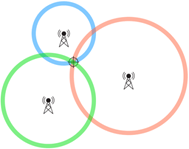
\includegraphics[width=\textwidth,height=\textheight,keepaspectratio]{triangulatie_gprs.png}
%https://www.google.com/search?tbs=simg:CAQSrQEJrrLXpgtW1nYaoQELELCMpwgaYgpgCAMSKJkIsBTyEoIDmgiDA5cIgQO5B4gDmj2dPaE0_1zO2J9A2-DP5M8U9yzcaMJJQwz9JWeZp5PeQ91p9B_1t-s-t57GaZYKqFkjHWNDErGPjWTFiDfGTdUPZPzFLx_1SAEDAsQjq7-CBoKCggIARIEyZLpqAwLEJ3twQkaGgoYCgZjaXJjbGXapYj2AwoKCC9tLzAxdmtsDA&sxsrf=ALeKk02ZKs3-33pizx_yPs1LYQ2NzzRrMw:1583058379858&q=trianguleren+mobiel&tbm=isch&sa=X&ved=2ahUKEwjJ_46DiPnnAhWNLewKHREFBhEQwg4oAHoECAcQKA
    \caption[Triangulatie bij GPRS]{De locatie (blauwe ster) wordt bepaald aan de hand van triangulatie met gsm-masten. De berekende schatting kan zich overal bevinden in het blauwe vlak}
    \label{fig:triangulatie_gprs}
\end{figure}
\pagebreak
\raggedbottom
\section{\IfLanguageName{dutch}{Ongunstige omstandigheden}{Unfavorable circumstances}}
De proof of concept moet blijven functioneren in ongunstige omstandigheden, zoals sneeuw en water. Het moet in staat zijn om te functioneren als GPS-ontvanger op een surfboard en als lawinepieper. In deze sectie wordt onderzocht aan welke voorwaarden de proof of concept moet voldoen.
\subsection{\IfLanguageName{dutch}{Water}{Water}}
Het grootste probleem voor GPS-ontvangers is dat ze niet kunnen functioneren onder water. Dit komt doordat de sterkte van het signaal te snel afneemt onder water. Hetzelfde geldt voor het mobiele netwerk, want beiden zijn elektromagnetische golven. \autocite{underwater} Er is ook een verschil tussen zout en zoetwater. Het zout in zeewater versterkt het geleidend effect waardoor GPS-signalen nog minder presteren in zeewater dan in zoetwater. Voor de proof of concept is dit geen struikelblok, indien het aan de zijkant van een surfboard wordt gemonteerd. Surfboards zijn zodanig gemaakt dat ze altijd blijven drijven, waardoor de proof of concept zal blijven functioneren naar behoren.
\subsection{\IfLanguageName{dutch}{Sneeuw}{Snow}}
In tegenstelling tot water, blijven GPS-signalen wel functioneren onder sneeuw tot een zekere diepte. Een GPS-signaal dat passeert door lawine puin zal onderworpen worden aan verschillende effecten zoals verzwakking, reflectie, verstrooiing, refractie, multipad en vervagen. (Zie figuur:\ref{fig:avalanche}) Sneeuw is net als water een geleidend materiaal, waardoor het (L1 band) GPS-signaal verzwakt. De verzwakking hangt af van de hoeveelheid water in de sneeuw. Een GPS-signaal kan bijvoorbeeld tot vierhonderd meter diep gaan bij sneeuw met een massadichtheid van 0.3 g/cm\textsuperscript{3}. Bij sneeuw waarbij het volumepercentage meer dan 1\% bedraagt kan het GPS-signaal slechts 3 meter diep doordringen.\autocite{avalanche_gps}
\begin{figure}
    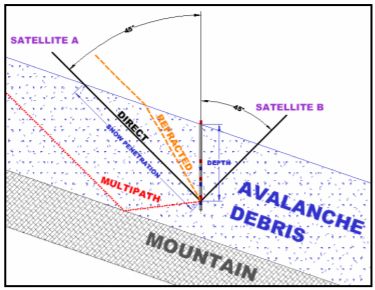
\includegraphics[width=\textwidth,height=\textheight,keepaspectratio]{avalanche.png}
    %https://www.researchgate.net/figure/Signal-Paths-in-Avalanche-Debris_fig1_253280455
    \caption[Negatieve invloed van refractie en weerkaatsing op GPS-signalen tijdens het penetreren van sneeuw]{\href{https://www.researchgate.net/figure/Signal-Paths-in-Avalanche-Debris_fig1_253280455}{Negatieve invloed van refractie en weerkaatsing op GPS-signalen tijdens het penetreren van sneeuw}}
    \label{fig:avalanche}
\end{figure}
\pagebreak